\documentclass[tikz,border=5mm,12pt]{standalone}
\usepackage[fontsize=16pt]{fontsize}
\usetikzlibrary{arrows.meta}
\usetikzlibrary{calc}

\newcommand\myfbox[1]{\fbox{#1\strut}}

\def\labelYsep{32pt}
\def\xsep{90mm}
\def\ysep{14mm}
\begin{document}
  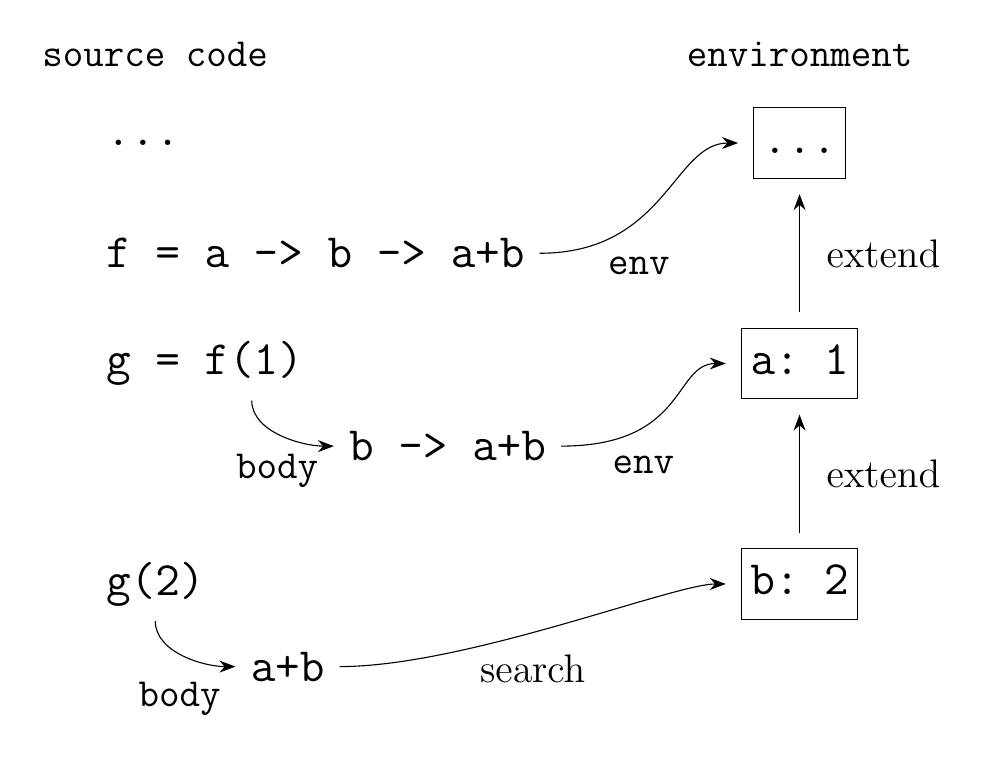
\begin{tikzpicture}[
    arrowtip/.style={
      -{Stealth[scale=1.2]}
    },
    upcurved/.style={
      in control={+(180:16mm)},
      out control={+(0:16mm)}
    },
    downcurved/.style={
      in control={+(180:4mm)},
      out control={+(-90:4mm)}
    },
    code/.style={
      anchor=west
    },
    subcode/.style={
      anchor=north west,below right=2mm
    }
  ]
    % left codes
    \node[code] at (-0.09*\xsep, \labelYsep) { \small\texttt{source code} };

    \node[code]           at (0*\xsep, 0*\ysep) { \texttt{...} };
    \node[code]    (OpB)  at (0*\xsep,-1*\ysep) { \texttt{f\ =\ a -> b -> a+b} };
    \node[code]    (OpC)  at (0*\xsep,-2*\ysep) { \texttt{g\ =\ f(1)} };
    \node[subcode] (OpCA) at (OpC.south east)   { \texttt{b\ ->\ a+b} };
    \node[code]    (OpD)  at (0*\xsep,-4*\ysep) { \texttt{g(2)} };
    \node[subcode] (OpDA) at (OpD.south east)   { \texttt{a+b} };

    % right environments
    \node at (1*\xsep, \labelYsep) { \small\texttt{environment} };

    \node (EnvA) at (1*\xsep, 0*\ysep) { \myfbox{\texttt{...}} };
    \node (EnvC) at (1*\xsep,-2*\ysep) { \myfbox{\texttt{a:\ 1}} };
    \node (EnvD) at (1*\xsep,-4*\ysep) { \myfbox{\texttt{b:\ 2}} };

    % arrows
    \coordinate (OpCR) at ($(OpC.south)+(6mm,0)$);
    \draw[downcurved,arrowtip] (OpCR)      to (OpCA.west);
    \path                      (OpCR)      -- (OpCA.west) node[midway,below=2mm,xshift=-2mm] { \small\texttt{body} };
    \draw[downcurved,arrowtip] (OpD.south) to (OpDA.west);
    \path                      (OpD.south) -- (OpDA.west) node[midway,below=3mm,xshift=-2mm] { \small\texttt{body} };

    \draw[arrowtip] (EnvC) -- (EnvA) node[midway,right=1.5mm] {\small extend};
    \draw[arrowtip] (EnvD) -- (EnvC) node[midway,right=1.5mm] {\small extend};

    \draw[upcurved,arrowtip] (OpB.east)  to (EnvA);
    \path                    (OpB.east)  -- (EnvA) node[midway,below=4mm] { \small\texttt{env} };
    \draw[upcurved,arrowtip] (OpCA.east) to (EnvC);
    \path                    (OpCA.east) -- (EnvC) node[midway,below=3mm] { \small\texttt{env} };
    \draw[upcurved,arrowtip] (OpDA.east) to (EnvD);
    \path                    (OpDA.east) -- (EnvD) node[midway,below=1mm] { \small search };
  \end{tikzpicture}
\end{document}
